\documentclass[12pt]{article}

\usepackage[letterpaper, hmargin=0.75in, vmargin=0.75in]{geometry}
\usepackage{float}
\usepackage{listings}
\usepackage{graphicx}
\usepackage{float}

\pagestyle{empty}

\title{ECE 459: Programming for Performance\\Assignment 3}
\author{Kenan Ali\\Lawrence Park}
\date{March 27, 2013}

% Code listing style
\lstset{frame=single}

\begin{document}

\maketitle

\section*{Part 1. Baseline Performance}
{\bf Majority of Runtime}
\\
\\
Using perf on lynch (ece459-1), and on a personal machine (Core 2 T5250) we see that a majority of the
runtime is spent in libm-2.16.so \_\_ieee754\_pow\_sse2 (~33.69\%), in libz.so.1.2.7 (~22.90\%), and in
test\_harness Model::morph(int, double, double, double) (~20.39\%). The following is an excerpt from perf
report:
\\
\begin{lstlisting}
Samples: 106K of event 'cycles', Event count (approx.): 97480443237
44.31% test_harness libm-2.17.so       [.] 0x0000000000014c2d
22.90% test_harness libz.so.1.2.7      [.] 0x0000000000003766
20.39% test_harness test_harness       [.] Model::morph(int, double,
                                             double, double)
3.79% test_harness libQtGui.so.4.8.4   [.] QVector2D::length() const
2.81% test_harness libpng15.so.15.13.0 [.] 0x0000000000022525
1.34% test_harness libm-2.17.so        [.] pow
\end{lstlisting}

(Since lynch was not resolving the symbols, we used the personal machine to verify that libm-2.16.so was
indeed calling \_\_ieee754\_pow\_sse2.)
\\
\\
Since we were only allowed to modify model.cpp, we needed to look at its structure to determine where
most of the time is spent within this function call. So we first ignored the library calls also dominating the
runtime. Upon inspecting morph() with perf annotate, we see a lot of Qt-related function calls, particularly in
the function's nested for-loops. These for-loops were determined to have the the critical loop with regards
to performance, so we knew that our optimizations had to target this.
The following excerpt shows a particularly hot portion of the critical loop within morph():
\newpage
\begin{lstlisting}
      |       QVector2D pQP(QP.y(), -QP.x()); 
      |                                                  
      |       // Calculate u, v 
      |       u = QVector2D::dotProduct(XP, QP) /  QP.lengthSquared(); 
 0.37 |   divsd  %xmm0,%xmm1   
12.98 |   movsd  %xmm1,-0x78(%rbp) 
      |       v = QVector2D::dotProduct(XP, pQP) / QP.length(); 
 0.58 | → callq  QVector2D::dotProduct(QVector2D const&,
                                 QVector2D const&)@plt 
      |   lea    -0x60(%rbp),%rdi 
      |   movsd  %xmm0,-0x88(%rbp) 
      | → callq  QVector2D::length() const@plt 
      |   movsd  -0x88(%rbp),%xmm2 
\end{lstlisting}

Finally, since the library function calls listed in perf report were significant chunks of the runtime, and
because we were only allowed to modify morph(), we had to determine if morph() calls the other
dominating components. By gaining this knowledge, we thought we might be able to address the amount of
time being spent in these library functions, hence improving performance further.
\\
\\
\\
{\bf Determine Library Callers}
\\
\\
After examining the morph function in model.cpp, we saw a lot of pow() calls on double value types. Since
the morph function is taking up a major part of the runtime, it can be reasonably assumed that the large
amount of time spent in the pow calculations is due to this. We can verify this by looking through perf
annotate on morph():
\newpage
\begin{lstlisting}
   inline const QPoint operator-(const QPoint &p1, const QPoint &p2) 
      	|       { return QPoint(p1.xp-p2.xp, p1.ypp2.yp); }                    
0.01 	|   sub    -0x94(%rbp),%r12d 
0.44 	|   movsd  -0x78(%rbp),%xmm0 
       	|   sub    -0x98(%rbp),%r13d 
0.00 	|   ucomis %xmm1,%xmm0 
0.48 	| ↓ jbe    204 
      	|   movsd0xbdf(%rip),%xmm0        
      	                    # 402958 <_IO_stdin_used+0xa8> 
0.00 	|   ucomis -0x78(%rbp),%xmm0 
0.36 	| ↓ ja     598 
       	|       else if(u <= 0) dist = sqrt(pow(X.x()
       	             - P.x(), 2.0) + pow(X.y() - P.y(), 2.0)); 
       	|204:   xorpd  %xmm3,%xmm3 
0.00 	|   ucomis -0x78(%rbp),%xmm3 
0.28 	| ↓ jae    580 
       	|       else dist = sqrt(pow(X.x() - Q.x(), 2.0)
       	             + pow(X.y() - Q.y(), 2.0)); 
       	|   mov    -0x98(%rbp),%eax 
       	|   sub    %r15d,%eax 
       	|   cvtsi2 %eax,%xmm1 
0.10 	|   mov    -0x94(%rbp),%eax 
0.00 	|   sub    -0x9c(%rbp),%eax 
       	|   cvtsi2 %eax,%xmm0 
0.13 	|230:   mulsd  %xmm0,%xmm0 
       	|   mulsd  %xmm1,%xmm1 
0.17 	|   addsd  %xmm0,%xmm1 
0.08 	|   sqrtsd %xmm1,%xmm0 
0.12 	|   ucomis %xmm0,%xmm0 
0.17 	| ↓ jp     838 
0.08 	|24a:   movsd  %xmm0,-0x78(%rbp)
\end{lstlisting}
To clarify the point: we see lots of XMM register use near pow() calls, so can be reasonably certain that a
significant portion of the SSE-based double math originates from morph().
\\
\\
Unfortunately, because the libz symbols were not found, we are unable to find out exactly where these calls
originate from. However, we can reason that they are not from morph() because morph carries out integer
and double math—not anything related to compression. It is likely that these calls are from the image
generation stage of the algorithm, and are therefore not a concern for us.
\newpage
\section*{Part 2. Improvements}
{\bf 1. Loop Parallelization via OpenMP}
\\
\\
After inspecting the baseline profile, we identified two for-loops in the morph() function in which exist the
critical loop. The critical loop is defined as embodying the program logic of the morphing algorithm, and performs floating-
point computations on variables. The iterations from this loop operate on individual pixels, and do not
mutate any global data. Parallelizing the execution of the loop via OpenMP involves minor synchronization
overhead. By using OpenMP, our implementation parallelizes the critical loop by flattening the two loops
(via the collapse clause). The following figure illustrates the changes made on top of the baseline
implementation:

\begin{figure}[H]%
\centering%
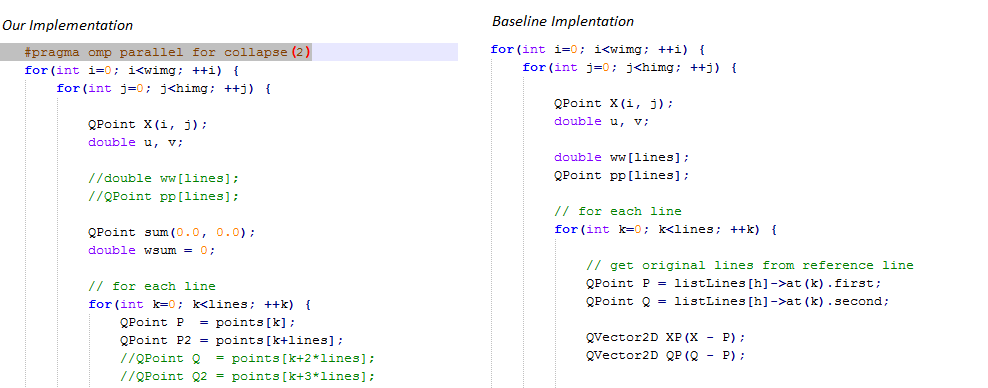
\includegraphics[scale=0.7]{codechange1.png}%
\caption{Use of OpenMP work-sharing construct on the critical loop}%
\label{fig:codechange1}%
\end{figure}


To profile the loop parallelization, we simply calculated the mean of the total runtime of baseline
implementation runs and the parallelized loop implementation. The following table illustrates the speedup
gained exclusively from the loop parallelization:\\
\\
\begin{center}
\begin{tabular}{l c r}
    Runtime & Baseline Code & Parallelized Code \\
    \hline
    Run 1 & 25.791 & 10.515\\
    Run 2 & 25.539 & 10.422\\
    Run 3 & 25.435 & 11.307\\
    Run 4 & 25.468 & 12.006\\
    Run 5 & 26.392 & 14.920\\
    Run 6 & 27.402 & 12.898\\
    \hline
    Average: & 26.004 & 12.011\\
\end{tabular}
\end{center}
\begin{center}Table 1. Profiled runtime of baseline code and parallelized code\end{center}
The average speed-up from the loop parallelization was over 2.16. This significant speedup can be attributed
to the fact that the critical loop of the morphing algorithm constitutes a majority of the total runtime, and
the algorithm is “embarrassingly parallel” due to the lack of data dependency between the loop iterations. 
As a result, parallelizing the critical loop incurs little synchronization overhead, and the workload to each
thread of execution is reduced by the number of physical cores on the host system.
\\
\\
{\bf 2. Pulling Redundant Code from the Critical Loop}
\\
\\
As previously discussed in this report, the critical loop located inside the morph() function is
responsible for the majority of the runtime. We noticed that the inner loop, which iterates over each
line in the global vector variables, performs various computations that could be done prior to
entering the critical loop. Specifically we separated the instantiation and accessing of various Qt 
data types from the math performed on them. The following figure illustrates the code changes made 
to the baseline code:
\begin{figure}[H]%
\centering%
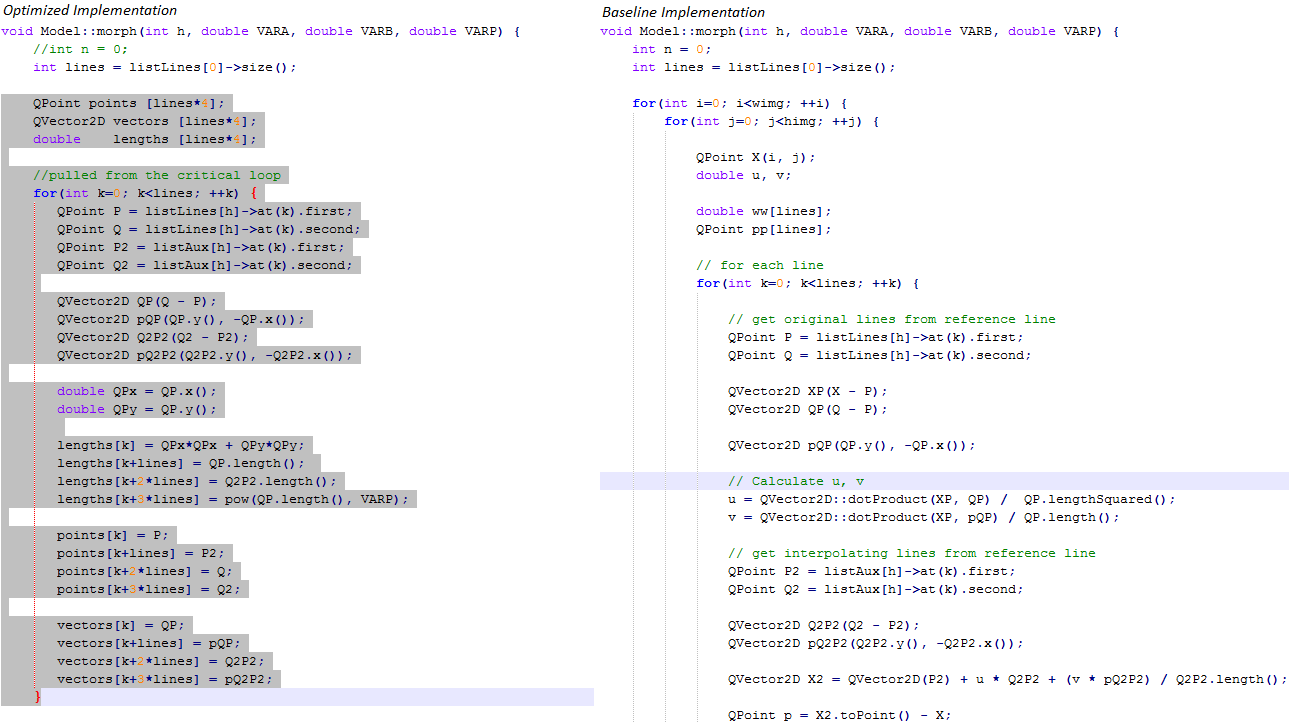
\includegraphics[scale=0.6]{codechange2.png}%
\caption{Use of OpenMP work-sharing construct on the critical loop}%
\label{fig:codechange2}%
\end{figure}


The code changes come from the realization that computations of inner loop variables, such as QP,
pQP, Q2P2, and pQ2P2, do not depend on the iterations of the critical loop. This means that the
baseline implementation repeatedly computes the same values for these variables in the critical loop.
By pre-computing the inner loop variables in a separate loop and storing the values on arrays, the
program runs faster without changing the semantics of the code. The following table tabulates the 
speedups gained by this change:
\\
\begin{center}
\begin{tabular}{l c r}
    Runtime & Baseline Code & Parallelized Code \\
    \hline
    Run 1 & 25.791 & 17.958\\
    Run 2 & 25.539 & 18.025\\
    Run 3 & 25.435 & 18.245\\
    Run 4 & 25.468 & 18.396\\
    Run 5 & 26.392 & 18.546\\
    Run 6 & 27.402 & 18.604\\
    \hline
    Average: & 26.004 & 18.296\\
\end{tabular}
\end{center}
\begin{center}Table 2. Profiled runtime of baseline code and modified code\end{center}
The speedup for the change was roughly 1.4. This modest speedup makes sense because the bulk of
time-consuming computations, such as the QVector2D dot product and floating point divisions, are
still taking place inside the critical loop. What was pulled from the critical loop constitutes
simpler and unnecessarily repeated operations, such as constructing QPoint and QVector2D objects. 
The semantics of the program remain unchanged because the pre-computed variables are independent 
from the loop iterations on i and j.
\end{document}
